The software landscape for fast solvers is fragmented, with comparisons between different techniques limited by the lack of availability of open-source parallel software. Algebraic methods are especially poorly represented, the only well supported open source parallel implementation being STRUMPACK \cite{ghyselsstrumpack}, which limits support to weakly admissable HODLR, and HSS matrices, but not strongly admissable $\mathcal{H}$ and $\mathcal{H}^2$ matrices. For the FMM there are a few more offerings, mainly from the ExaFMM project, who have produced ExaFMM, an MPI accelerated analytical FMM \cite{exafmm}, as well as ExaFMM-T, an OpenMP accelerated single-node black box FMM \cite{wang2021exafmm}.

Yokota and co-workers offer one of the few comparisons between software packages \cite{yokota2015fast}, by comparing STRUMPACK and ExaFMM for the calculation of the Laplace problem (\ref{eq:two_box_calc:sec_1_2}) for $N$ randomly distributed charges $\{ q_i\}_{i=1}^N$ placed in a unit cube, $[0, 1]^3$, in $\mathbb{R}^3$. We extend their study, by comparing both with ExaFMM-T\footnote{Our experiments are available at \url{https://github.com/skailasa/phd-thesis/code/ch_2/}}. Thus providing an overview of algebraic, semi-analytical and analytical FMM software implementations. Our experiments were performed on a single 32 core AMD Ryzed Threadripper 3970X processor, where we set OMP\_NUM\_THREADS=1, to avoid oversubscription in ExaFMM and STRUMPACK, and keep results comparable. We note that Yokota et. al report only the matrix vector product time, however we also report the total time for computation, including the time to set up all data structures. We reason that it is a fairer evaluation between radically different approaches, and more reflective of a user's perspective when evaluating a library for use own use. Runtimes are plotted in figure (\ref{fig:sec_2_0:software_comparison}a), alongside peak memory usage in figure (\ref{fig:sec_2_0:software_comparison}b). 

We report STRUMPACK fails to converge rapidly ($\leq$1 hour) for the Laplace problem when the number of particles, $N$, exceeded $10^5$, which lies in contrast to previously reported results \cite{yokota2015fast}. This is the result of two major issues. Firstly, we calculate the matrix elements of (\ref{eq:two_box_calc:sec_1_2}) naively, without any SIMD optimisations as used in the highest performing FMM implementations such as \cite{wang2021exafmm}. Secondly, the HSS matrix approximation is not strictly appropriate for a (\ref{eq:two_box_calc:sec_1_2}), as it assumes adjacent nodes are low-rank. Thus, interactions between adjacent nodes are compressed less than they ought to be, with the rank of interactions between adjacent nodes growing at higher levels. However we believe that our experiments, with relatively small problem sizes, are reflective of typical average user - who would similarly implement an initial naive kernel advanced code generation tools. In this case, we find that the difference in runtime performance for $N=10^4$ between STRUMPACK and ExaFMM spans two orders of magnitude, for ExaFMM-T this grows to three orders of magnitude. 

As expected The kernel independent ExaFMM-T uses more memory than the analytical ExaFMM. The growth rate in memory use for the HSS matrices is clearly greater 

\begin{figure}%
    \centering
    \subfloat[\centering Runtime]{{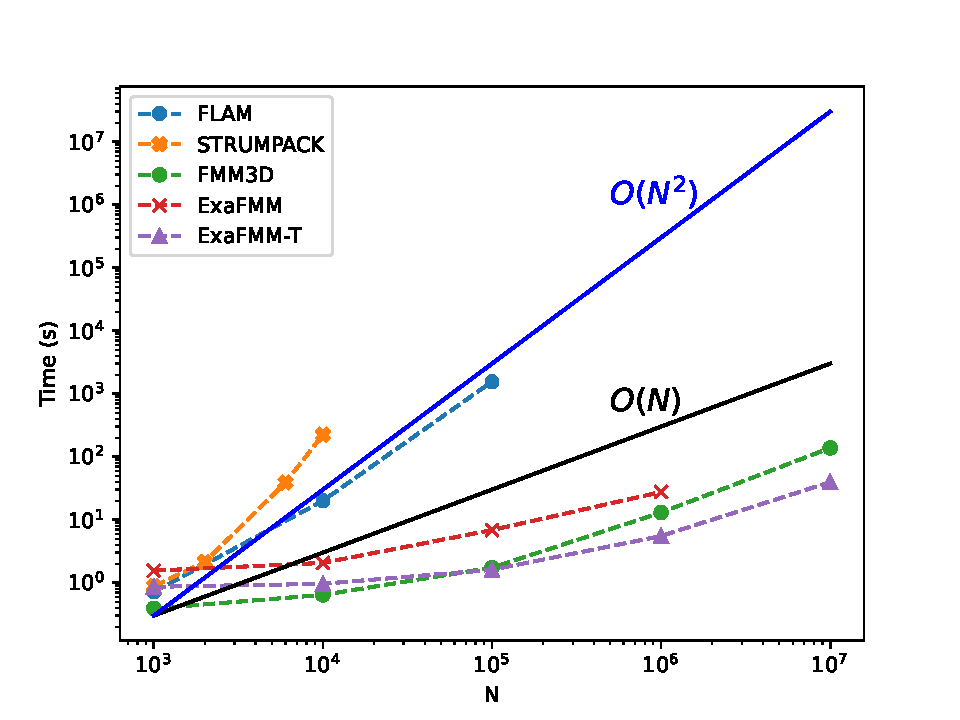
\includegraphics[width=6cm]{ch_2/runtime.pdf} }}%
    \qquad
    \subfloat[\centering Peak Memory Usage]{{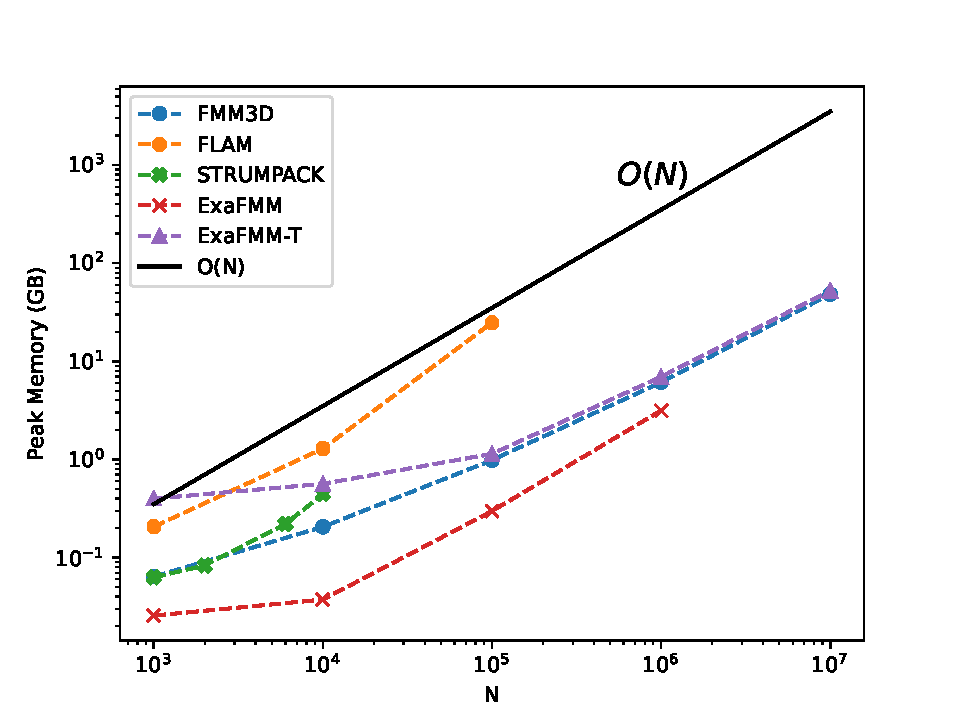
\includegraphics[width=6cm]{ch_2/memory.pdf} }}
    \caption{A comparison of runtime and memory usage to compute (\ref{eq:two_box_calc:sec_1_2}) using STRUMPACK, ExaFMM and ExaFMM-T.  STRUMPACK fails to converge for $N \geq 10^5$ in under an hour.}
    \label{fig:sec_2_0:software_comparison}%
\end{figure}

Yokota et. al. compare the matrix vector products of (\ref{eq:two_box_calc:sec_1_2}) performed by the \gls{FMM} using the ExaFMM package \cite{exafmm} and HSS factorisations using the STRUMPACK package \cite{rouet2016distributed}. 

These methods are not directly comparable, as the HSS method is only weakly admissible, however it constitutes on of the few studies to directly compare the efficacy of analytical and algebraic methods. They observe that the FMM converges approximately O(10) faster, with up to $O(1000)$ smaller memory footprint for (\ref{eq:eq:two_box_calc:sec_1_2}) in $R^3$ when computed on a single node.

- Get more examples and data on the difficulties faced by researchers for research software.

- Explain how the software goal of this research is to design software that can scale from a laptop to the latest supercomputing cluster.

~ 1 page